\documentclass[11pt, oneside]{article} 
\usepackage{geometry}
\geometry{letterpaper} 
\usepackage{graphicx}
	
\usepackage{amssymb}
\usepackage{amsmath}
\usepackage{parskip}
\usepackage{color}
\usepackage{hyperref}

\graphicspath{{/Users/telliott_admin/Dropbox/Tex/png/}}
% \begin{center} 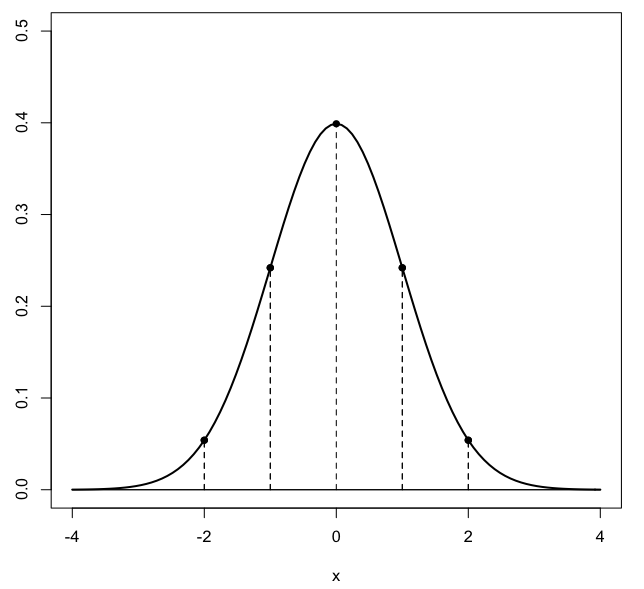
\includegraphics [scale=0.4] {gauss3.png} \end{center}

\title{Ellipse}
\date{}

\begin{document}
\maketitle
\Large

\label{sec:Ellipse_geometry}

\section*{construction}

\begin{center} 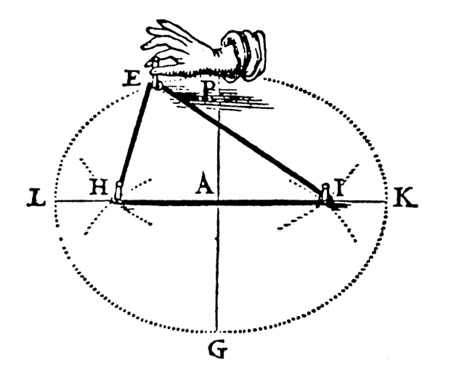
\includegraphics [scale=0.4] {ellipse_acheson.png} \end{center}
Learning how to draw an ellipse using two pins and a circular piece of string holding a pencil is an early adventure in mathematics.  The ellipse is the set of all points whose combined distance to the two pins (foci) is the same.

The drawing is reproduced from a 17th century book in Acheson (see the References).

\begin{center} 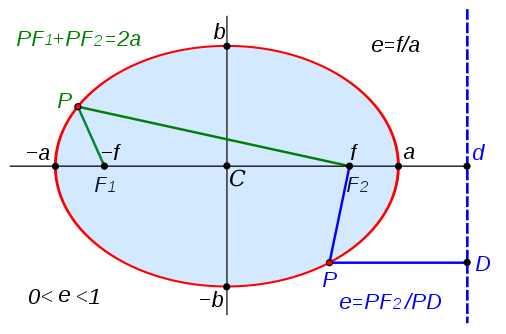
\includegraphics [scale=0.45] {ellipse_wikipedia.png} \end{center}
The pin positions with respect to the origin or center are called the foci, lying at the points shown in the figure as ($\pm f,0$).

We will use the notation $c$:  the focus in the first quadrant is at the point $(c,0)$.

The lengths of the axes (called semi-major and semi-minor) are usually labeled $a$ and $b$.  

Consider the situation when the pencil is at the point $P = (0,a)$.  The distance to the left focus is $c+a$, so the length $L$ of the string is twice that
\[ L = 2(c+a) \]
The combined distance from each point on the ellipse to the two foci is the length of the string minus the distance between the two foci
\[ L - 2c = 2(c+a) - 2c = 2a \]

\subsection*{standard equation}
We learn in algebra that the equation for an ellipse is
\[ \frac{x^2}{a^2} + \frac{y^2}{b^2} = 1 \]
We will derive this equation below.

The relation of $a$ and $c$ to $b$ can be seen from the point $Q=(0,b)$ (see previous figure) where the combined distance to the two foci is just
\[ QF_1 + QF_2 \]
From what we said above the distance is $2a$, but Pythagoras also gives us
\[ QF_1 + QF_2 = 2a = 2\sqrt{b^2 + c^2} \]
so
\[ b^2 + c^2 = a^2 \]
\[ c^2 = a^2 - b^2 \]
Given $a$ and $b$ one can then find $c$ easily.

Here are three ellipses drawn with the same center.
\begin{center} 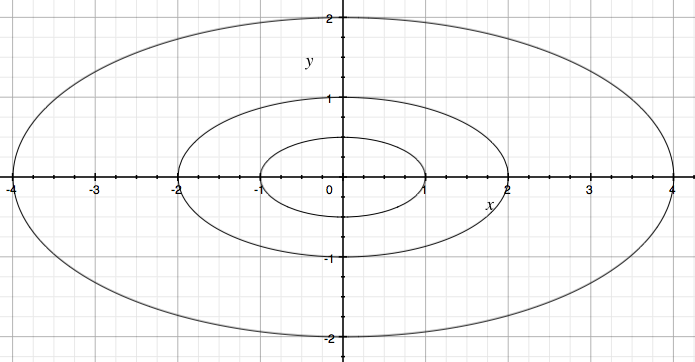
\includegraphics [scale=0.35] {ellipses_three.png} \end{center}
The difference is an adjustment in the value on the right-hand side of the equation
\[ \frac{x^2}{a^2} + \frac{y^2}{b^2} = r^2 \]

where $r = \{ 1/2,1,2 \}$.  This is equivalent to scaling both $a$ and $b$ by the same factor of $r$
\[ \frac{x^2}{(ra)^2} + \frac{y^2}{(rb)^2} = 1 = (\frac{x/a}{r})^2 +  (\frac{y/b}{r})^2 \]

When $r=2$ we need to make the string a bit less than twice as long, because the length $c$ is also involved:
\[ \frac{L_2}{L_1} = \frac{ra + c}{a + c} \]

\subsection*{parametrization}
An alternative view is the one below, which shows (black curves) the upper half of two circles of radius $r=1$ and $r=2$ and an ellipse whose equation is 
\[ \frac{x^2}{2^2} + \frac{y^2}{1} = 1 \]

\begin{center} 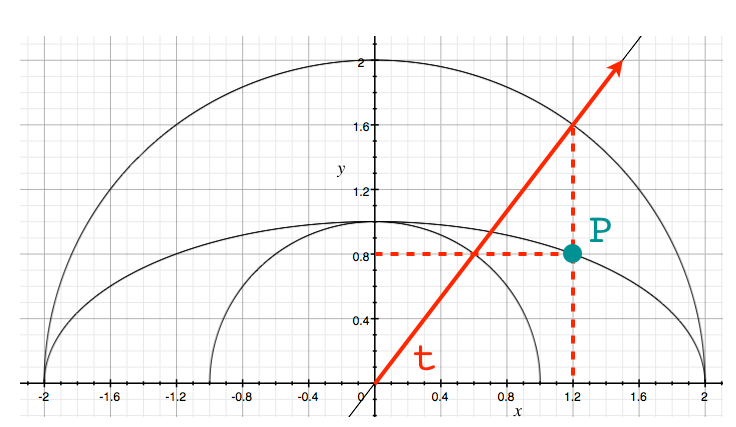
\includegraphics [scale=0.4] {p_ellipse.png} \end{center}
Here $a=2$ and $b=1$.

The standard parametrization of the ellipse is
\[ x = a \cos t \]
\[ y = b \sin t \]
which I had trouble visualizing, until I drew the picture.  The thing is that the parameter $t$ is \emph{not} the angle that a ray to $P$ makes with the $x$-axis, as it is for the circle.  Instead, to find the $x$ value of $P$ corresponding to $t$, we extend the ray with angle $t$ to the larger circle, with radius $a$, where we read off the $x$-value as 
\[ x=a \cos t \]
We go back to find the intersection of the same ray with the small circle to get 
\[ y = b \sin t \]

The algebraic way to do this is to show that the parametrization is equivalent to the original formulation
\[ x^2 = a^2 \cos^2 t \]
\[ y^2 = b^2 \sin^2 t \]
\[ \frac{x^2}{a^2} + \frac{y^2}{b^2} = \cos^2 t + \sin^2 t = 1 \]
as expected.

\subsection*{Derivation of the equation of the ellipse}
Although it is a bit tedious, it's a reasonable exercise to derive the equation of the ellipse from the geometric constraint.  Recall that $a$ is the length of the semi-major axis and $c$ the distance to each of the foci from the origin.  

\begin{center} 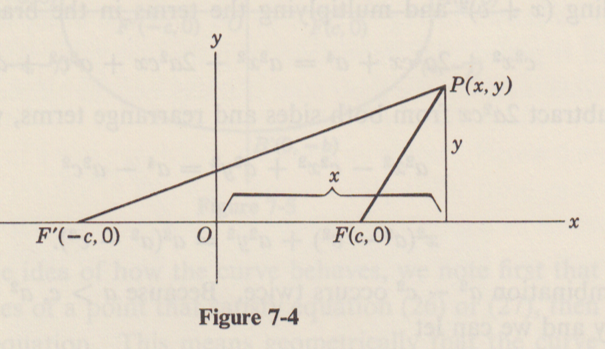
\includegraphics [scale=0.4] {Kline_7_4.png} \end{center}

For any point $x,y$ on the ellipse, the distance to the focus in the first quadrant is
\[ \sqrt{(x - c)^2 + y^2} \]
and combined distances to both foci are equal to $2a$ so
\[ 2a = \sqrt{(x + c)^2 + y^2} + \sqrt{(x - c)^2 + y^2} \]

Now we just do some algebra.  Pick one square root and rearrange
\[ \sqrt{(x - c)^2 + y^2} = 2a - \sqrt{(x + c)^2 + y^2} \]
Square both sides
\[ (x - c)^2 + y^2 = 4a^2 - 4a \sqrt{(x + c)^2 + y^2} + (x+c)^2 + y^2 \]
Cancel $y^2$
\[ (x - c)^2 = 4a^2 - 4a \sqrt{(x + c)^2 + y^2} + (x+c)^2 \]
But
\[ (x+c)^2 - (x-c)^2 = 4xc \]
so
\[ 0 = 4a^2 - 4a \sqrt{(x + c)^2 + y^2} + 4xc \]
\[ a^2 + xc = a \sqrt{(x + c)^2 + y^2} \]
Square again
\[ a^4 + 2a^2xc + x^2c^2 = a^2(x^2 + 2xc + c^2 + y^2) \]
\[ a^4 + 2a^2xc + x^2c^2 = a^2x^2 + 2a^2xc + a^2c^2 + a^2y^2 \]
Cancel $2a^2xc$
\[ a^4 + x^2c^2 = a^2x^2 + a^2c^2 + a^2y^2 \]
Gather terms
\[ a^4 - a^2c^2 = a^2x^2 - x^2c^2 + a^2y^2 \]
\[ a^2(a^2 - c^2) = x^2(a^2 - c^2) + a^2y^2 \]
Recall that $b^2 = a^2 - c^2$
\[ b^2a^2 = b^2x^2 +a^2y^2  \]
Divide by $a^2b^2$
\[ \frac{x^2}{a^2} + \frac{y^2}{b^2} = 1  \]

\hypertarget{rotation}{}
\subsection*{rotation}

Let's return to the diagram of the ellipse with two bounding circles of radius $a$ and radius $b$.  There is a new diagram below.  Consider the coordinates of the point $P=(x,y)$ (the red dot in the first quadrant) as functions of the angle $t$.  As we said, $t$ is \emph{not} the angle of a ray from the origin to $P$.

Draw a ray (blue dotted line) from the origin makes an angle $t$ with the $x$-axis.  As before, extend the ray to the outer circle.  The radius is $a$, the angle is $t$, and
\[ a \cos t = x \]
This is the parametrization of the ellipse introduced previously.
\begin{center} 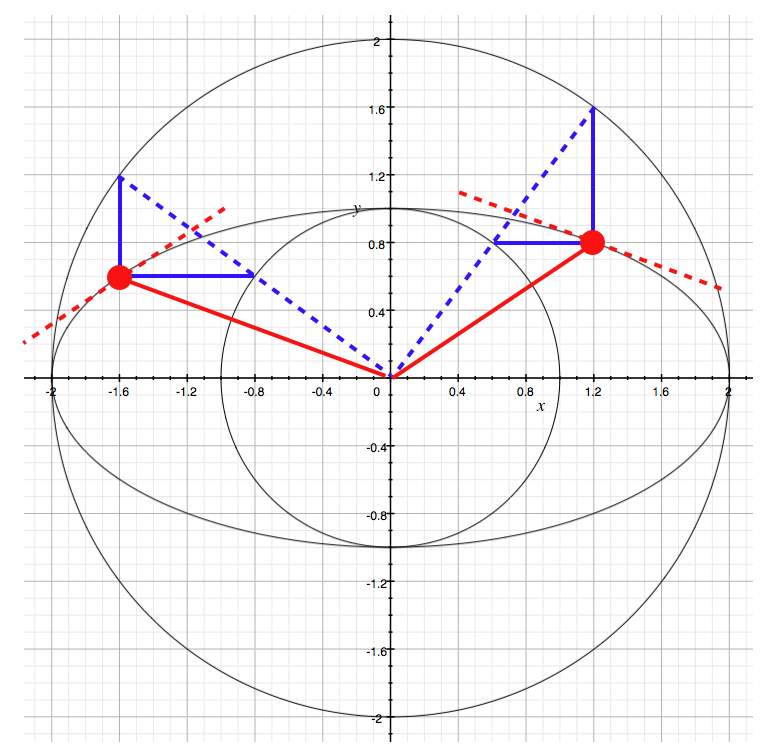
\includegraphics [scale=0.3] {ellipse_fancy.png} \end{center}

The ray drawn with angle $t$ has the same $x$-intercept with the outer circle as our point $P$ on the ellipse.  Similarly, the intercept of the ray with the inner circle has the same $y$-value as the point $P$ on the ellipse.

We estimate the point $P=(1.2,0.8)=(6/5,4/5)$.  Using our algebraic equation:
\[ \frac{x^2}{a^2} + \frac{y^2}{b^2} = 1 \]

Recall that $a=2$ and $b=1$ so
\[ x^2 + 4y^2 = 4 \]

Plugging in for $x^2$ and $y^2$ we get
\[ \frac{36}{25} + 4 \ (\frac{16}{25}) = \frac{100}{25} = 4 \]
as expected.  Reading off the intercepts for the ray with angle $t$ (dotted blue line) with the outer circle, we have the point $(1.2,1.6)$ at a distance $2$ from the origin.  Thus,
\[ \frac{1.2}{2} = 0.6 = \cos t \]
\[ t \approx 0.927\ \text{rad} \approx 53^{\circ} \]

Looking again at the figure, we want to consider what happens for the angle $u = t + \pi/2$.  This is the dotted blue ray in the second quadrant.

We might calculate the values of sine and cosine for $u$, but notice that if we view $u$ as a vector, its \emph{dot product} with $t$ must be equal to zero.  The coordinates of the intercept of the rotated vector with the outer circle are $(-1.6,1.2)$, so the cosine of the angle $u$ is
\[ \cos u = -0.8 \]
\[ u \approx 2.498 = t + \frac{\pi}{2} \ \text{rad} \approx 143^{\circ} \]
We confirm that 
\[ 2.498 - 0.927 = 1.57 = \frac{\pi}{2} \]

The coordinates of the point on the ellipse are $(-1.6,0.6)$, which we check against the formula
\[ x^2 + 4y^2 = 4 \]
\[ (1.6)^2 + 4(0.6)^2 = 2.56 + 4(0.36) = 4 \]
(no clean fractions this for this one).

\subsection*{tangent}
Finally, and this is really the crucial result:

the vector to the point, call it $Q$, on the ellipse (red dot in the second quadrant) is the \emph{tangent to the ellipse} for the point $P$ in the first quadrant.

How did this happen?  Recall what we did.  We had 
\[ x = a \cos t \]
\[ y = b \sin t \]

The rotated point $Q = (x',y')$ is
\[ x' = a \cos (t + \frac{\pi}{2}) \]
\[ y' = b \sin (t + \frac{\pi}{2}) \]

\begin{center} 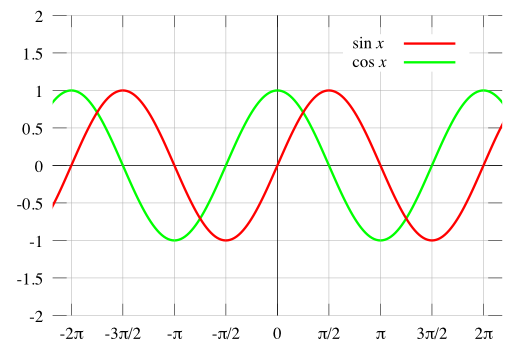
\includegraphics [scale=0.4] {sine_cosine_wikipedia.png} \end{center}
Sine is like cosine, but shifted to the right by $\pi/2$
\[ \cos \theta = \sin (\theta + \frac{\pi}{2}) \]
\[ \sin \theta = - \cos (\theta + \frac{\pi}{2}) \]
So
\[ x' = a \cos (t + \frac{\pi}{2}) = -a \sin t \]
\[ y' = b \sin (t + \frac{\pi}{2}) = b \cos t \]

Let's look at the position vector, which can be written $\mathbf{r}(t)$, since it's a function of the angle $t$ or the time, but we will just use $\mathbf{r}$.  It has components $x$ and $y$.

\[ \mathbf{r} = \ \langle x,y \rangle \ = \ \langle a \cos t,b \sin t \rangle \ \]

Now, the tangent to the ellipse is precisely the direction in which a particle at $(x,y)$ is currently moving on the ellipse.  The tangent vector points in the same direction as the velocity vector, but $\mathbf{v}$ is just the time-derivative of the position vector.
\[ \mathbf{v} = \frac{d\mathbf{r}}{dt} \]
\[ = \ \langle \frac{dx}{dt}, \frac{dy}{dt} \rangle \]
\[ = \ \langle -a \sin t,b \cos t \rangle \]
\[ = \ \langle x',y' \rangle \]

These two methods --- using the time-derivative as the tangent, and rotation of $t$ by $\pi/2$ --- generate the same vector.  And that's the point.   :)

\subsection*{Starbird}
Here is a neat approach to the ellipse that I saw in one of Michael Starbird's lectures.

Imagine a glass cylinder, shown here in cross-section and colored black.  The cylinder has been sliced through at an angle by a plane, and we suppose a flat piece of glass in the shape of an ellipse is glued between the two halves.  

The elongated region in red (formed at the plane of the cut) is the ellipse, and the cylinder is oriented so that at each horizontal position going across the page, the two points on the ellipse are at the same vertical position.  We see the plane of the cut edge-on.
\begin{center} 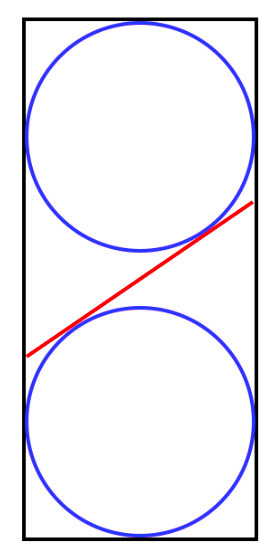
\includegraphics [scale=0.35] {cylinder_slant1.png} \end{center}
Two spheres that fit snugly inside the cylinder lie above and below the ellipse, just touching it.  The planar surface of the ellipse is tangent to the spheres, touching each one at a single point.

We claim that the points where the spheres touch the ellipse are the foci of the ellipse.

By the nature of the construction, the two spheres just fit inside the cylinder.  That means the intersection where the spheres touch the cylinder is a circle, the lower one is shown with a dotted blue line in the next figure.
\begin{center} 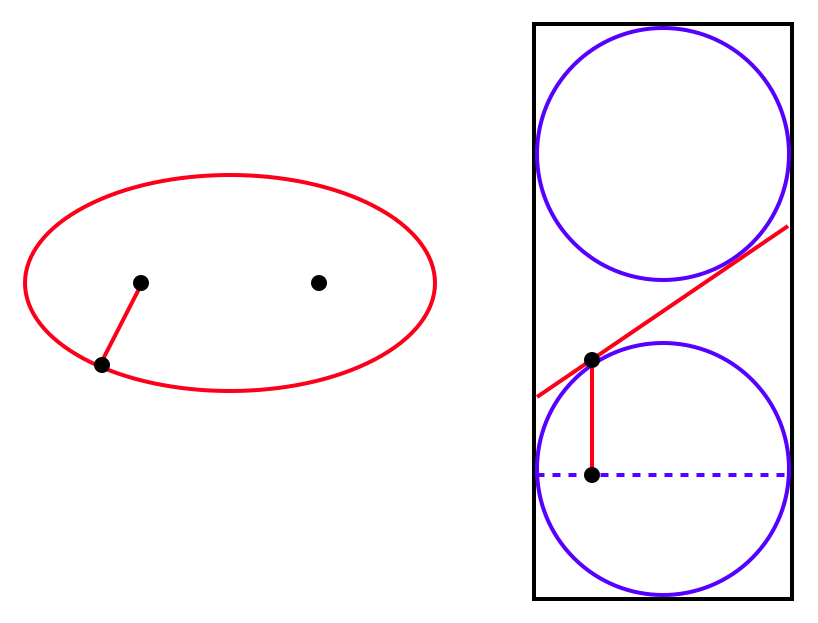
\includegraphics [scale=0.35] {cylinder_slant2.png} \end{center}
Now consider any point on the ellipse.  On the left, we see one point on the ellipse together with two interior points we claim are foci, with a line drawn from our point to one of the foci. 

We said that this point is the point where the ellipse touches the lower sphere.  We conclude that the line we've drawn from the edge of the ellipse to the focus is a tangent to the sphere. 

A second tangent of interest is the perpendicular dropped vertically down the surface of the cylinder, shown in the right panel. Since they are both tangents, this line is the same length as line to the focus.

But the construction, and this equality, holds for any point on the ellipse, as shown in the next figure.
\begin{center} 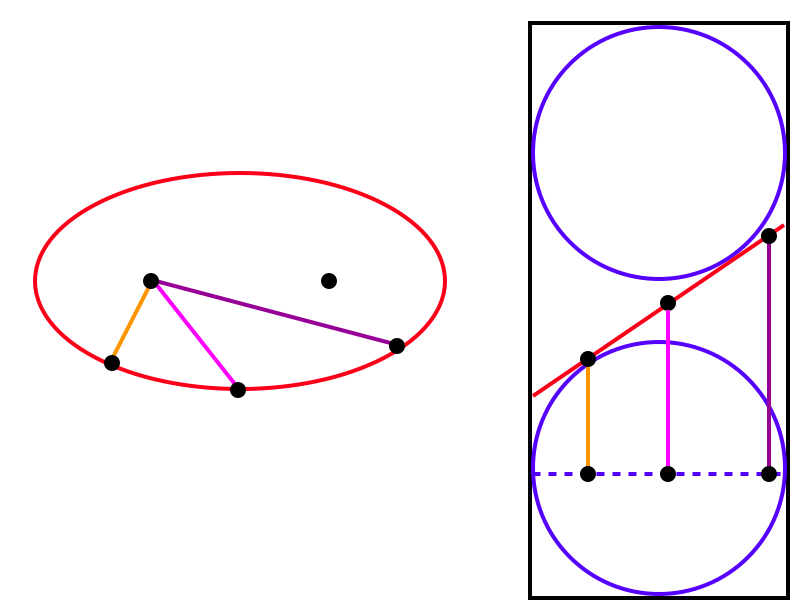
\includegraphics [scale=0.35] {cylinder_slant3.png} \end{center}
Finally, this is true for both spheres (below). The sum of the perpendicular tangents for any point is a constant. 
\begin{center} 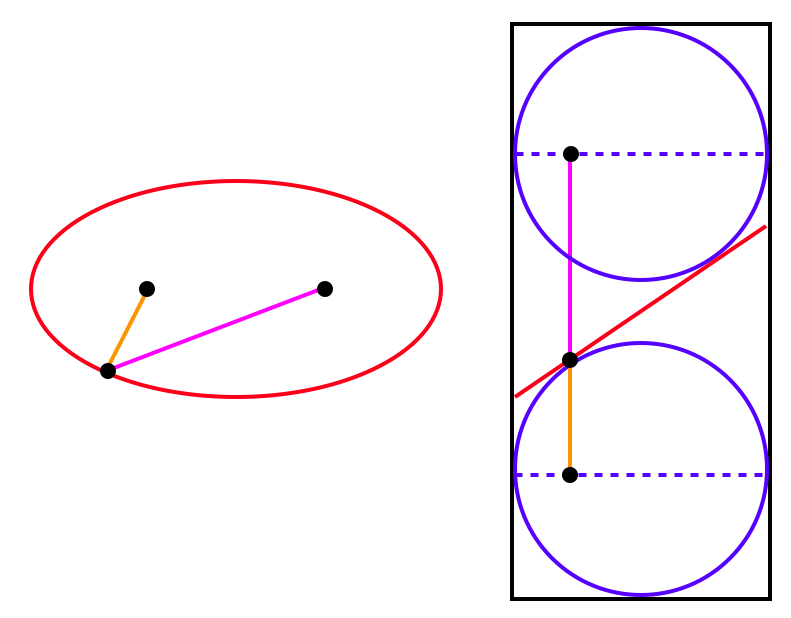
\includegraphics [scale=0.35] {cylinder_slant4.png} \end{center}
Thus, the points where the spheres touch the ellipse are its foci, because the sum of the distances to any point on the ellipse, which is equal to the sum of the vertical tangents, is a constant.

\begin{center} 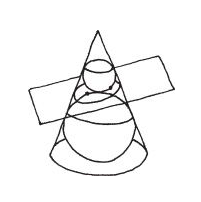
\includegraphics [scale=0.6] {ellipse_cone.png} \end{center}

According to Lockhart, the same argument can be used to prove that the cross sections of a cone are ellipses (which seems strange at first since we've been demonstrating that the cross-sections of cylinders are also ellipses).

\end{document}